\begin{flushleft}
    \huge
    \textbf{2. Analysis}
    \vspace{0.1cm}

    \Large
    \begin{enumerate}
        \item {\Large Statement of Investigation} \\
            \large
            I plan to investigate Machine Learning by developing a survival simulation environment 
            in which an Agent will be controlled by a Machine Learning algorithm. 
            The survival simulation will present multiple challenges towards the agent 
            in order to provide a complex problem for it to solve. 
            The key question I aim to answer with this investigation is:

            \vspace{0.3cm}

            \begin{center}
            \textbf{Can you train a Machine Learning algorithm to survive in a pseudo random, open-world environment?}
            \end{center}

            \vspace{0.3cm}

            I find this question to be quite interesting because there is multiple layers of complexity to it, 
            with several different problems to solve. Answering the question will require me to dive headfirst into 
            Machine Learning picking things up as fast as possible.

            \pagebreak
        \item {\Large Background} \\

        \item {\Large Expert} \\

        \item {\Large Initial Research} \\

            \pagebreak
        \item {\Large Prototype} \\
            \large
            Before starting my Prototype I had to decide upon a short list of objectives I wanted to 
            complete/investigate as part of it. These boiled down to a few things:

            \vspace{0.2cm}
            \begin{enumerate}
                \item Terrain Generation
                \item Displaying the Generated Terrain using a Grahics Library
                \item Matrix and Vector implementation
            \end{enumerate}
            \vspace{0.2cm}

            For my Prototype, I first created a GitHub Repository, available here: 
            
            \vspace{0.1cm}
            \centerline{\textit{https://github.com/TheTacBanana/CompSciNEAPrototype}}
            \vspace{0.1cm}

            I had created a hierarchy of importance for development in my head, visualized using this flow diagram:

            \begin{center}
                \begin{tikzpicture}
                    \matrix (m)[matrix of nodes, column  sep=0.5cm,row  sep=0.5cm, align=center, nodes={rectangle,draw, anchor=center} ]{
                        |[block]| Creating a window with Graphics Library &  |[block]| Display Generated Terrain \\   
                        |[block]| Generate Terrain using a pseudorandom algorithm &  |[block]| Store Terrain to 2d List \\
                        |[block]| Create a Matrix Data Structure & |[block]| Create a Vector Data Structure which inherits from Matrix \\
                        |[block]| Create Operation Methods for the Data Structure & \\
                    };
                    \path [>=latex,->] (m-1-1) edge (m-1-2);
                    \path [>=latex,<-] (m-1-2) edge (m-2-2);
                    \path [>=latex,->] (m-2-1) edge (m-2-2);
                    \path [>=latex,->] (m-3-1) edge (m-3-2);
                    \path [>=latex,->] (m-3-1) edge (m-4-1);
                \end{tikzpicture}
            \end{center}

            I decided to use Python for developing my Prototype, this seemed like a good fit due to me 
            having lots of experience with the language. Python is a Dynamically Typed and Interpretted 
            language which makes it versatile for protyping and fast, iterative development.
            
            \vspace{0.5cm}

            Starting from the begining of my hierarchy I installed Pygame using \textit{pip} and started creating a window.
            This was a relatively simple task only taking a few lines:
            \vspace{0.5cm}

            \normalsize
            \begin{lstlisting}[language=Python]
import pygame

simSize = 128
gridSize = 2

window = pygame.display.set_mode((simSize * gridSize, simSize * gridSize))
pygame.display.set_caption("Procedural Generation")

running = True
while running == True:
  for event in pygame.event.get():
    if event.type == pygame.QUIT:
      running = False
            \end{lstlisting}

            \vspace{0.5cm}

            \large
            This creates a window like this: \\ 
            \vspace{0.5cm}
            \centerline{
\includegraphics{Images/Prototype/CreateWindowExample.PNG}}

            \vspace{0.5cm}

            Following the hierarchy I then added noise generation by generating random numbers and 
            assigning them to a 2d List. Shown here: 
            
            \normalsize\begin{lstlisting}[language=Python]
def GenerateMap(self, seed):
    random.seed(seed)
    for y in range(0, self.arraySize):
        for x in range(0, self.arraySize):
            self.heightArray[x][y] = round(random.random(),2)
            \end{lstlisting}

            \vspace{0.5cm}

            \large
            After creating some code to draw squares based upon the random value, I ended up with this 
            random array of Black-White squares:\\
            \vspace{0.5cm}
            \centerline{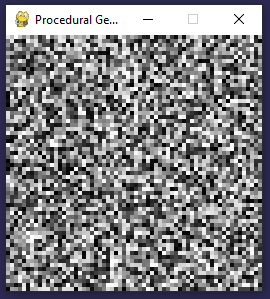
\includegraphics{Images/Prototype/RandomNoiseExample.PNG}}

            \vspace{0.5cm}

            This was a good start, but didnt really look like terrain yet. As part of my research I came 
            across simple algorithms to turn random noise into usable 2d terrain. I decided to implement
            these algorithms. They are relatively short and didnt take too much time to implement. I've
            named the two algorithms UpDownNeutralGen and Average.

            \vspace{1cm}

            {\Large UpDownNeutralGen Method} \\
            \vspace{0.25cm}

            The UpDownNeutralGen method takes a tile, and considers every tile around it. It sums the tile 
            which are greater than, less than, or within a certain range of the tile height. And then pulls
            the selected tile in the direction which has the highest precedence. As an example, here are some
            randomly generated values

            \begin{center}
                \begin{tabular}{| M{0.75cm} | M{0.75cm} | M{0.75cm} |}
                    \hline
                    0.71 & 0.19 & 0.3 \\ [0.75cm]
                    \hline
                    0.46 & 0.26 & 0.82 \\ [0.75cm]
                    \hline
                    0.63 & 0.35 & 0.05 \\ [0.75cm]
                    \hline
                \end{tabular}
            \end{center}

            If we count the surrounding values into corresponding Higher, Lower and Neutral we get: \\

            \begin{center}
                \begin{tabular}{| M{2cm} | M{2cm} | M{2cm} |}
                    \hline
                    Higher & Lower & Neutral \\ [0.25cm]
                    \hline
                    4 & 1 & 3 \\ [0.25cm]
                    \hline
                \end{tabular}
            \end{center}

            \vspace{0.5cm}

            This leads us to calculating the \textit{pullValue}, respectively for each case:
            \begin{center}
                $Up -> pullValue = upTiles * 0.09$ \\
                $Down -> pullValue = upTiles * -0.08$ \\
                $Neutral -> pullValue = 0$ \\
                \vspace{0.5cm}
                $Value[x][y] \pluseq pullValue$\\
            \end{center}
            

            \vspace{1cm}

            {\Large Average Method}

            \pagebreak
        \item {\Large Objectives} \\
            \large
            Taking into account my Prototype and Interview, I have formed a list of objectives I feel to be most 
            appropriate for my Investigation.
            If all completed they will form a complete solution which will answer my Investigations question.
            Below is the list of objectives split into 6 key sections:

            \begin{enumerate}
                \item User Input
                    \begin{enumerate}
                        \item Read Parameters from a Json formatted file
                        \item Check Parameters fall within a certain range to prevent errors
                        \item Give user option to load Neural Network Training progress
                    \end{enumerate}
                \item Simulation
                    \begin{enumerate}
                        \item Utilise Perlin Noise to generate a 2d List of terrain heights
                        \item Store Terrain Heights in a Tile Data Type
                        \item Utilise Threading to generate Terrain Faster
                        \item Display terrain to a pygame window
                        \item Map ranges of terrain heights to specific colour bands
                        \item Utilise Poisson Disc Sampling to generate objects for the Agent to interact with
                        \item Implement enemies which use basic pathfinding to traverse towards the player
                        \item Generate multiple enemies upon starting the simulation
                        \item Allow the enemies to attack the Agent
                    \end{enumerate}   
                \item Agent
                    \begin{enumerate}
                        \item Implement Movement options for the Agent
                        \item Implement the ability to pick up the generated Objects
                        \item Implement the ability to attack the generated enemies
                        \item Create methods to sample the terrain around the Agent
                        \item Create methods to convert the sampled Tiles into a grayscale input vector for a neural network
                        \item Create reward methods to reward the agent given the terrain samples and action
                    \end{enumerate}   
                \item Matrix Class
                    \begin{enumerate}
                        \item Implement a Dynamic Matrix Class with appropriate Operations such as:
                            \begin{enumerate}
                                \item Multiplication
                                \item Addition
                                \item Subtraction
                                \item Transpose
                                \item Sum
                                \item Select Row/Column
                            \end{enumerate}
                        \item Create appropriate errors to throw when utilising methods the incorrect way
                    \end{enumerate}   
                \item Deep Q Learning
                    \begin{enumerate}
                        \item Dynamically create a Dual Neural Network model based upon loaded parameters
                        \item Implement an Abstract Class for Activation Functions
                        \item Implement Activation Functions inheriting from the Abstract Class such as:
                        \begin{enumerate}
                            \item ReLu
                            \item Sigmoid
                            \item SoftMax
                        \end{enumerate}
                        \item Create methods to Forward Propagate the neural network
                        \item Create methods to calculate the loss of the network using the Bellman Equation
                        \item Create methods to Back Propagate calculated error through the neural network
                        \item Create methods to update weights and biases within the network to converge on a well trained network
                        \item Utilise the outlined Matrix class to perform the mathematical operations in the specified methods
                        \item Implement Load and Save Methods to save progress in training
                        \item Implement a Double Ended Queue/Deque Data Type
                        \item Implement Experience Replay utilising the Deque Data Type to increase training accuracy
                    \end{enumerate}   
                \item Data Logger
                    \begin{enumerate}
                        \item Be able to create a Data Logger class to log data points across training
                        \item Be able to create a Data Structure for the Data Logger
                        \item Allow multiple types specified types for a single parameter
                        \item When adding a new Data Point the Logger will check it to make sure it matches the given Data Structure
                        \item Implement a Heap Data Type
                        \item Implement a Heap sort using the Heap Data Type
                        \item Be able to sort by a parameter in the Data Structure
                        \item Be able to select a single parameter from the data points
                        \item Implement Load and Save Functions to save progress during training
                    \end{enumerate}   
            \end{enumerate}


    \end{enumerate}
\end{flushleft}